\documentclass{article}
\usepackage[T1]{fontenc}
\usepackage[scaled=0.94]{helvet}
\renewcommand{\familydefault}{\sfdefault}
\usepackage{tikz}
\usetikzlibrary{arrows.meta}
\pagestyle{empty}
\setlength{\parindent}{0pt}
\setlength{\topskip}{0pt}
\setlength{\parskip}{0pt}
\definecolor{ink}{HTML}{262B30}
\definecolor{bluew}{HTML}{356D96}
\definecolor{loserfill}{HTML}{D7DCE0}
\definecolor{loseredge}{HTML}{8E969C}
\definecolor{unreadfill}{HTML}{EEF1F3}
\definecolor{unreadt}{HTML}{9BA3AA}
\definecolor{edgec}{HTML}{AAB1B7}
\definecolor{edgepale}{HTML}{D8DEE2}
\definecolor{ptrc}{HTML}{303840}
\definecolor{exh}{HTML}{C44C3C}
\definecolor{muted}{HTML}{6E777E}
\definecolor{container}{HTML}{C5CCD1}
\definecolor{containerpale}{HTML}{E1E5E8}
\definecolor{palebg}{HTML}{F7F8F9}
\definecolor{gapbg}{HTML}{FBFCFC}
\definecolor{white}{HTML}{FFFFFF}
\newcommand{\numfont}{\sffamily\bfseries\fontsize{6.15}{7}\selectfont}
\newcommand{\labelfont}{\sffamily\fontsize{5.7}{6.6}\selectfont}
\newcommand{\captionfont}{\sffamily\fontsize{6.05}{7.1}\selectfont}
\newcommand{\idfont}{\sffamily\fontsize{6.35}{7.4}\selectfont}
\newcommand{\headfont}{\sffamily\bfseries\fontsize{8}{9.2}\selectfont}
\newcommand{\titlefont}{\sffamily\bfseries\fontsize{7.15}{8.3}\selectfont}
\begin{document}
\pdfhorigin=0bp
\pdfvorigin=0bp
\setbox0=\hbox{%
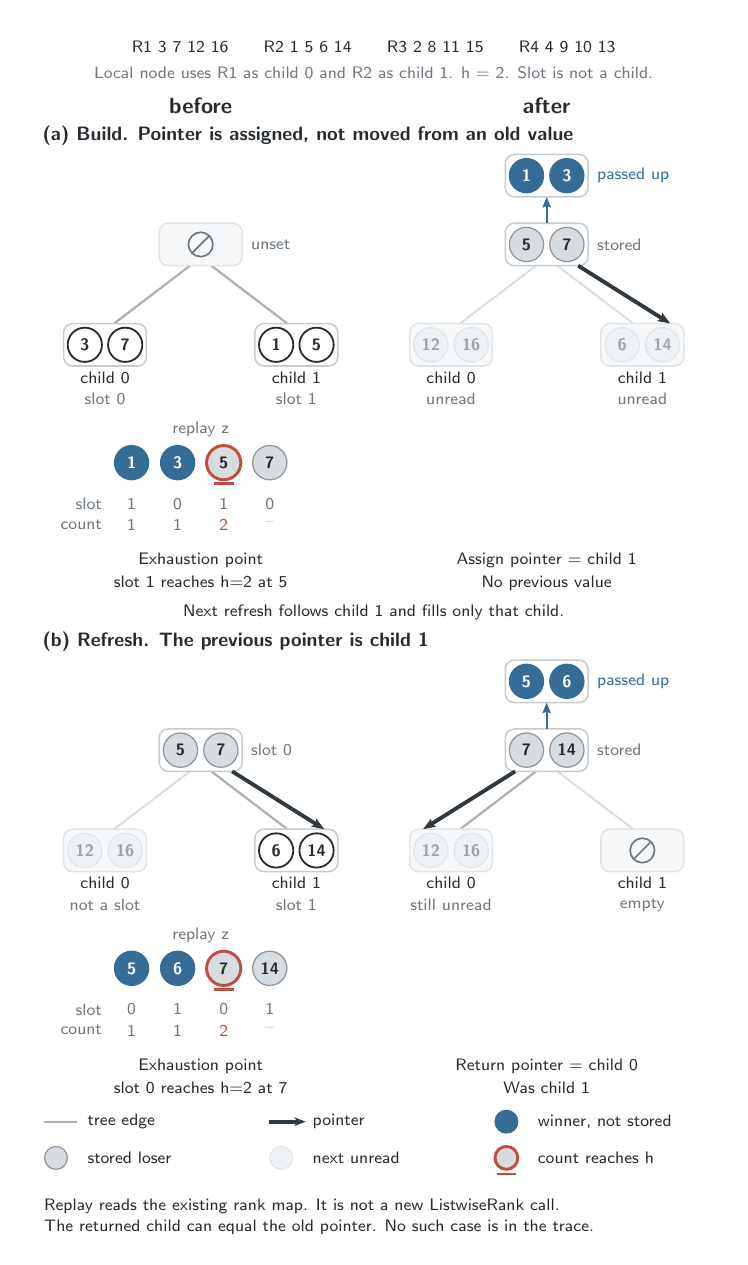
\begin{tikzpicture}[x=1mm,y=1mm,every node/.style={inner sep=0pt,outer sep=0pt}]
\node[inner sep=0pt, anchor=north, align=center, font=\idfont, text=ink] at (43.942,151.840) {R1  3 7 12 16\qquad R2  1 5 6 14\qquad R3  2 8 11 15\qquad R4  4 9 10 13};
\node[inner sep=0pt, anchor=north, align=center, font=\captionfont, text=muted] at (43.942,148.540) {Local node uses R1 as child 0 and R2 as child 1. h = 2. Slot is not a child.};
\node[inner sep=0pt, anchor=north, align=center, font=\headfont, text=ink] at (21.971,144.540) {before};
\node[inner sep=0pt, anchor=north, align=center, font=\headfont, text=ink] at (65.913,144.540) {after};
\node[inner sep=0pt, anchor=north west, align=left, font=\titlefont, text=ink] at (1.900,141.040) {(a) Build. Pointer is assigned, not moved from an old value};
\draw[line width=0.8pt, draw=edgec, line cap=butt] (20.621,123.310) -- (10.971,115.960);
\draw[line width=0.8pt, draw=edgec, line cap=butt] (23.321,123.310) -- (32.971,115.960);
\draw[rounded corners=1.150mm, line width=0.55pt, draw=containerpale, fill=palebg] (16.711,123.310) rectangle (27.231,128.700);
\draw[line width=0.6pt, draw=muted] (21.971,126.005) circle (1.550mm);
\draw[line width=0.6pt, draw=muted] (20.921,124.955) -- (23.021,127.055);
\node[inner sep=0pt, anchor=west, align=left, font=\labelfont, text=muted] at (28.381,126.005) {unset};
\draw[rounded corners=1.150mm, line width=0.55pt, draw=container, fill=white] (4.561,110.570) rectangle (15.081,115.960);
\draw[line width=0.65pt, draw=ink, fill=white] (7.256,113.265) circle (2.175mm);
\node[inner sep=0pt, font=\numfont, text=ink] at (7.256,113.265) {3};
\draw[line width=0.65pt, draw=ink, fill=white] (12.386,113.265) circle (2.175mm);
\node[inner sep=0pt, font=\numfont, text=ink] at (12.386,113.265) {7};
\draw[rounded corners=1.150mm, line width=0.55pt, draw=container, fill=white] (28.861,110.570) rectangle (39.381,115.960);
\draw[line width=0.65pt, draw=ink, fill=white] (31.556,113.265) circle (2.175mm);
\node[inner sep=0pt, font=\numfont, text=ink] at (31.556,113.265) {1};
\draw[line width=0.65pt, draw=ink, fill=white] (36.686,113.265) circle (2.175mm);
\node[inner sep=0pt, font=\numfont, text=ink] at (36.686,113.265) {5};
\node[inner sep=0pt, anchor=north, align=center, font=\labelfont, text=ink] at (9.821,109.870) {child 0};
\node[inner sep=0pt, anchor=north, align=center, font=\labelfont, text=muted] at (9.821,107.120) {slot 0};
\node[inner sep=0pt, anchor=north, align=center, font=\labelfont, text=ink] at (34.121,109.870) {child 1};
\node[inner sep=0pt, anchor=north, align=center, font=\labelfont, text=muted] at (34.121,107.120) {slot 1};
\node[inner sep=0pt, anchor=north, align=center, font=\labelfont, text=muted] at (21.971,103.470) {replay z};
\node[inner sep=0pt, anchor=north east, align=left, font=\labelfont, text=muted] at (9.421,93.770) {slot};
\node[inner sep=0pt, anchor=north east, align=left, font=\labelfont, text=muted] at (9.421,91.070) {count};
\draw[line width=0.4pt, draw=bluew, fill=bluew] (13.196,98.295) circle (2.175mm);
\node[inner sep=0pt, font=\numfont, text=white] at (13.196,98.295) {1};
\node[inner sep=0pt, anchor=north, align=center, font=\labelfont, text=muted] at (13.196,93.770) {1};
\node[inner sep=0pt, anchor=north, align=center, font=\labelfont, text=muted] at (13.196,91.070) {1};
\draw[line width=0.4pt, draw=bluew, fill=bluew] (19.046,98.295) circle (2.175mm);
\node[inner sep=0pt, font=\numfont, text=white] at (19.046,98.295) {3};
\node[inner sep=0pt, anchor=north, align=center, font=\labelfont, text=muted] at (19.046,93.770) {0};
\node[inner sep=0pt, anchor=north, align=center, font=\labelfont, text=muted] at (19.046,91.070) {1};
\draw[line width=1.05pt, draw=exh, fill=loserfill] (24.896,98.295) circle (2.175mm);
\node[inner sep=0pt, font=\numfont, text=ink] at (24.896,98.295) {5};
\node[inner sep=0pt, anchor=north, align=center, font=\labelfont, text=muted] at (24.896,93.770) {1};
\node[inner sep=0pt, anchor=north, align=center, font=\labelfont, text=exh] at (24.896,91.070) {2};
\draw[line width=0.95pt, draw=exh, line cap=butt] (23.646,95.640) -- (26.146,95.640);
\draw[line width=0.45pt, draw=loseredge, fill=loserfill] (30.746,98.295) circle (2.175mm);
\node[inner sep=0pt, font=\numfont, text=ink] at (30.746,98.295) {7};
\node[inner sep=0pt, anchor=north, align=center, font=\labelfont, text=muted] at (30.746,93.770) {0};
\node[inner sep=0pt, anchor=north, align=center, font=\labelfont, text=edgepale] at (30.746,91.070) {--};
\node[inner sep=0pt, anchor=north, align=center, font=\captionfont, text=ink] at (21.971,86.820) {Exhaustion point};
\node[inner sep=0pt, anchor=north, align=center, font=\captionfont, text=ink] at (21.971,83.920) {slot 1 reaches h=2 at 5};
\draw[line width=0.7pt, draw=edgepale, line cap=butt] (64.563,123.310) -- (54.913,115.960);
\draw[line width=0.7pt, draw=edgepale, line cap=butt] (67.263,123.310) -- (76.913,115.960);
\draw[rounded corners=1.150mm, line width=0.55pt, draw=container, fill=white] (60.653,132.050) rectangle (71.173,137.440);
\draw[line width=0.4pt, draw=bluew, fill=bluew] (63.348,134.745) circle (2.175mm);
\node[inner sep=0pt, font=\numfont, text=white] at (63.348,134.745) {1};
\draw[line width=0.4pt, draw=bluew, fill=bluew] (68.478,134.745) circle (2.175mm);
\node[inner sep=0pt, font=\numfont, text=white] at (68.478,134.745) {3};
\node[inner sep=0pt, anchor=west, align=left, font=\labelfont, text=bluew] at (72.323,134.745) {passed up};
\draw[rounded corners=1.150mm, line width=0.55pt, draw=container, fill=white] (60.653,123.310) rectangle (71.173,128.700);
\draw[line width=0.45pt, draw=loseredge, fill=loserfill] (63.348,126.005) circle (2.175mm);
\node[inner sep=0pt, font=\numfont, text=ink] at (63.348,126.005) {5};
\draw[line width=0.45pt, draw=loseredge, fill=loserfill] (68.478,126.005) circle (2.175mm);
\node[inner sep=0pt, font=\numfont, text=ink] at (68.478,126.005) {7};
\node[inner sep=0pt, anchor=west, align=left, font=\labelfont, text=muted] at (72.323,126.005) {stored};
\draw[rounded corners=1.150mm, line width=0.55pt, draw=containerpale, fill=palebg] (48.503,110.570) rectangle (59.023,115.960);
\draw[line width=0.45pt, draw=containerpale, fill=unreadfill] (51.198,113.265) circle (2.175mm);
\node[inner sep=0pt, font=\numfont, text=unreadt] at (51.198,113.265) {12};
\draw[line width=0.45pt, draw=containerpale, fill=unreadfill] (56.328,113.265) circle (2.175mm);
\node[inner sep=0pt, font=\numfont, text=unreadt] at (56.328,113.265) {16};
\draw[rounded corners=1.150mm, line width=0.55pt, draw=containerpale, fill=palebg] (72.803,110.570) rectangle (83.323,115.960);
\draw[line width=0.45pt, draw=containerpale, fill=unreadfill] (75.498,113.265) circle (2.175mm);
\node[inner sep=0pt, font=\numfont, text=unreadt] at (75.498,113.265) {6};
\draw[line width=0.45pt, draw=containerpale, fill=unreadfill] (80.628,113.265) circle (2.175mm);
\node[inner sep=0pt, font=\numfont, text=unreadt] at (80.628,113.265) {14};
\node[inner sep=0pt, anchor=north, align=center, font=\labelfont, text=ink] at (53.763,109.870) {child 0};
\node[inner sep=0pt, anchor=north, align=center, font=\labelfont, text=muted] at (53.763,107.120) {unread};
\node[inner sep=0pt, anchor=north, align=center, font=\labelfont, text=ink] at (78.063,109.870) {child 1};
\node[inner sep=0pt, anchor=north, align=center, font=\labelfont, text=muted] at (78.063,107.120) {unread};
\draw[line width=0.8pt, draw=bluew, line cap=butt, -{Stealth[length=1.35mm, width=1.05mm, inset=0.2mm]}] (65.913,128.700) -- (65.913,132.050);
\draw[line width=1.4pt, draw=ptrc, line cap=butt, -{Stealth[length=1.55mm, width=1.15mm, inset=0.25mm]}] (69.913,123.310) -- (81.613,115.960);
\node[inner sep=0pt, anchor=north, align=center, font=\captionfont, text=ink] at (65.913,86.820) {Assign pointer = child 1};
\node[inner sep=0pt, anchor=north, align=center, font=\captionfont, text=ink] at (65.913,83.920) {No previous value};
\node[inner sep=0pt, anchor=north, align=center, font=\captionfont, text=ink] at (43.942,80.220) {Next refresh follows child 1 and fills only that child.};
\node[inner sep=0pt, anchor=north west, align=left, font=\titlefont, text=ink] at (1.900,76.820) {(b) Refresh. The previous pointer is child 1};
\draw[line width=0.7pt, draw=edgepale, line cap=butt] (20.621,59.090) -- (10.971,51.740);
\draw[line width=0.8pt, draw=edgec, line cap=butt] (23.321,59.090) -- (32.971,51.740);
\draw[rounded corners=1.150mm, line width=0.55pt, draw=container, fill=white] (16.711,59.090) rectangle (27.231,64.480);
\draw[line width=0.45pt, draw=loseredge, fill=loserfill] (19.406,61.785) circle (2.175mm);
\node[inner sep=0pt, font=\numfont, text=ink] at (19.406,61.785) {5};
\draw[line width=0.45pt, draw=loseredge, fill=loserfill] (24.536,61.785) circle (2.175mm);
\node[inner sep=0pt, font=\numfont, text=ink] at (24.536,61.785) {7};
\node[inner sep=0pt, anchor=west, align=left, font=\labelfont, text=muted] at (28.381,61.785) {slot 0};
\draw[rounded corners=1.150mm, line width=0.55pt, draw=containerpale, fill=palebg] (4.561,46.350) rectangle (15.081,51.740);
\draw[line width=0.45pt, draw=containerpale, fill=unreadfill] (7.256,49.045) circle (2.175mm);
\node[inner sep=0pt, font=\numfont, text=unreadt] at (7.256,49.045) {12};
\draw[line width=0.45pt, draw=containerpale, fill=unreadfill] (12.386,49.045) circle (2.175mm);
\node[inner sep=0pt, font=\numfont, text=unreadt] at (12.386,49.045) {16};
\draw[rounded corners=1.150mm, line width=0.55pt, draw=container, fill=white] (28.861,46.350) rectangle (39.381,51.740);
\draw[line width=0.65pt, draw=ink, fill=white] (31.556,49.045) circle (2.175mm);
\node[inner sep=0pt, font=\numfont, text=ink] at (31.556,49.045) {6};
\draw[line width=0.65pt, draw=ink, fill=white] (36.686,49.045) circle (2.175mm);
\node[inner sep=0pt, font=\numfont, text=ink] at (36.686,49.045) {14};
\node[inner sep=0pt, anchor=north, align=center, font=\labelfont, text=ink] at (9.821,45.650) {child 0};
\node[inner sep=0pt, anchor=north, align=center, font=\labelfont, text=muted] at (9.821,42.900) {not a slot};
\node[inner sep=0pt, anchor=north, align=center, font=\labelfont, text=ink] at (34.121,45.650) {child 1};
\node[inner sep=0pt, anchor=north, align=center, font=\labelfont, text=muted] at (34.121,42.900) {slot 1};
\draw[line width=1.4pt, draw=ptrc, line cap=butt, -{Stealth[length=1.55mm, width=1.15mm, inset=0.25mm]}] (25.971,59.090) -- (37.671,51.740);
\node[inner sep=0pt, anchor=north, align=center, font=\labelfont, text=muted] at (21.971,39.250) {replay z};
\node[inner sep=0pt, anchor=north east, align=left, font=\labelfont, text=muted] at (9.421,29.550) {slot};
\node[inner sep=0pt, anchor=north east, align=left, font=\labelfont, text=muted] at (9.421,26.850) {count};
\draw[line width=0.4pt, draw=bluew, fill=bluew] (13.196,34.075) circle (2.175mm);
\node[inner sep=0pt, font=\numfont, text=white] at (13.196,34.075) {5};
\node[inner sep=0pt, anchor=north, align=center, font=\labelfont, text=muted] at (13.196,29.550) {0};
\node[inner sep=0pt, anchor=north, align=center, font=\labelfont, text=muted] at (13.196,26.850) {1};
\draw[line width=0.4pt, draw=bluew, fill=bluew] (19.046,34.075) circle (2.175mm);
\node[inner sep=0pt, font=\numfont, text=white] at (19.046,34.075) {6};
\node[inner sep=0pt, anchor=north, align=center, font=\labelfont, text=muted] at (19.046,29.550) {1};
\node[inner sep=0pt, anchor=north, align=center, font=\labelfont, text=muted] at (19.046,26.850) {1};
\draw[line width=1.05pt, draw=exh, fill=loserfill] (24.896,34.075) circle (2.175mm);
\node[inner sep=0pt, font=\numfont, text=ink] at (24.896,34.075) {7};
\node[inner sep=0pt, anchor=north, align=center, font=\labelfont, text=muted] at (24.896,29.550) {0};
\node[inner sep=0pt, anchor=north, align=center, font=\labelfont, text=exh] at (24.896,26.850) {2};
\draw[line width=0.95pt, draw=exh, line cap=butt] (23.646,31.420) -- (26.146,31.420);
\draw[line width=0.45pt, draw=loseredge, fill=loserfill] (30.746,34.075) circle (2.175mm);
\node[inner sep=0pt, font=\numfont, text=ink] at (30.746,34.075) {14};
\node[inner sep=0pt, anchor=north, align=center, font=\labelfont, text=muted] at (30.746,29.550) {1};
\node[inner sep=0pt, anchor=north, align=center, font=\labelfont, text=edgepale] at (30.746,26.850) {--};
\node[inner sep=0pt, anchor=north, align=center, font=\captionfont, text=ink] at (21.971,22.600) {Exhaustion point};
\node[inner sep=0pt, anchor=north, align=center, font=\captionfont, text=ink] at (21.971,19.700) {slot 0 reaches h=2 at 7};
\draw[line width=0.8pt, draw=edgec, line cap=butt] (64.563,59.090) -- (54.913,51.740);
\draw[line width=0.7pt, draw=edgepale, line cap=butt] (67.263,59.090) -- (76.913,51.740);
\draw[rounded corners=1.150mm, line width=0.55pt, draw=container, fill=white] (60.653,67.830) rectangle (71.173,73.220);
\draw[line width=0.4pt, draw=bluew, fill=bluew] (63.348,70.525) circle (2.175mm);
\node[inner sep=0pt, font=\numfont, text=white] at (63.348,70.525) {5};
\draw[line width=0.4pt, draw=bluew, fill=bluew] (68.478,70.525) circle (2.175mm);
\node[inner sep=0pt, font=\numfont, text=white] at (68.478,70.525) {6};
\node[inner sep=0pt, anchor=west, align=left, font=\labelfont, text=bluew] at (72.323,70.525) {passed up};
\draw[rounded corners=1.150mm, line width=0.55pt, draw=container, fill=white] (60.653,59.090) rectangle (71.173,64.480);
\draw[line width=0.45pt, draw=loseredge, fill=loserfill] (63.348,61.785) circle (2.175mm);
\node[inner sep=0pt, font=\numfont, text=ink] at (63.348,61.785) {7};
\draw[line width=0.45pt, draw=loseredge, fill=loserfill] (68.478,61.785) circle (2.175mm);
\node[inner sep=0pt, font=\numfont, text=ink] at (68.478,61.785) {14};
\node[inner sep=0pt, anchor=west, align=left, font=\labelfont, text=muted] at (72.323,61.785) {stored};
\draw[rounded corners=1.150mm, line width=0.55pt, draw=containerpale, fill=palebg] (48.503,46.350) rectangle (59.023,51.740);
\draw[line width=0.45pt, draw=containerpale, fill=unreadfill] (51.198,49.045) circle (2.175mm);
\node[inner sep=0pt, font=\numfont, text=unreadt] at (51.198,49.045) {12};
\draw[line width=0.45pt, draw=containerpale, fill=unreadfill] (56.328,49.045) circle (2.175mm);
\node[inner sep=0pt, font=\numfont, text=unreadt] at (56.328,49.045) {16};
\draw[rounded corners=1.150mm, line width=0.55pt, draw=containerpale, fill=palebg] (72.803,46.350) rectangle (83.323,51.740);
\draw[line width=0.6pt, draw=muted] (78.063,49.045) circle (1.550mm);
\draw[line width=0.6pt, draw=muted] (77.013,47.995) -- (79.113,50.095);
\node[inner sep=0pt, anchor=north, align=center, font=\labelfont, text=ink] at (53.763,45.650) {child 0};
\node[inner sep=0pt, anchor=north, align=center, font=\labelfont, text=muted] at (53.763,42.900) {still unread};
\node[inner sep=0pt, anchor=north, align=center, font=\labelfont, text=ink] at (78.063,45.650) {child 1};
\node[inner sep=0pt, anchor=north, align=center, font=\labelfont, text=muted] at (78.063,42.900) {empty};
\draw[line width=0.8pt, draw=bluew, line cap=butt, -{Stealth[length=1.35mm, width=1.05mm, inset=0.2mm]}] (65.913,64.480) -- (65.913,67.830);
\draw[line width=1.4pt, draw=ptrc, line cap=butt, -{Stealth[length=1.55mm, width=1.15mm, inset=0.25mm]}] (61.913,59.090) -- (50.213,51.740);
\node[inner sep=0pt, anchor=north, align=center, font=\captionfont, text=ink] at (65.913,22.600) {Return pointer = child 0};
\node[inner sep=0pt, anchor=north, align=center, font=\captionfont, text=ink] at (65.913,19.700) {Was child 1};
\draw[line width=0.8pt, draw=edgec] (2.100,14.600) -- (6.300,14.600);
\node[inner sep=0pt, anchor=west, align=left, font=\captionfont, text=ink] at (7.600,14.600) {tree edge};
\draw[line width=1.4pt, draw=ptrc, -{Stealth[length=1.45mm, width=1.1mm]}] (30.700,14.600) -- (35.300,14.600);
\node[inner sep=0pt, anchor=west, align=left, font=\captionfont, text=ink] at (36.200,14.600) {pointer};
\draw[line width=0.4pt, draw=bluew, fill=bluew] (60.800,14.600) circle (1.45mm);
\node[inner sep=0pt, anchor=west, align=left, font=\captionfont, text=ink] at (64.800,14.600) {winner, not stored};
\draw[line width=0.45pt, draw=loseredge, fill=loserfill] (3.600,10.000) circle (1.45mm);
\node[inner sep=0pt, anchor=west, align=left, font=\captionfont, text=ink] at (7.600,10.000) {stored loser};
\draw[line width=0.45pt, draw=containerpale, fill=unreadfill] (32.200,10.000) circle (1.45mm);
\node[inner sep=0pt, anchor=west, align=left, font=\captionfont, text=ink] at (36.200,10.000) {next unread};
\draw[line width=1.05pt, draw=exh, fill=loserfill] (60.800,10.000) circle (1.45mm);
\draw[line width=0.95pt, draw=exh] (59.600,7.950) -- (62.000,7.950);
\node[inner sep=0pt, anchor=west, align=left, font=\captionfont, text=ink] at (64.800,10.000) {count reaches h};
\node[inner sep=0pt, anchor=north west, align=left, font=\captionfont, text=ink] at (2.100,4.800) {Replay reads the existing rank map. It is not a new ListwiseRank call.};
\node[inner sep=0pt, anchor=north west, align=left, font=\captionfont, text=ink] at (2.100,2.100) {The returned child can equal the old pointer. No such case is in the trace.};
\path[use as bounding box] (0,0) rectangle (87.884,153.540);
\end{tikzpicture}%
}
\pdfpagewidth=\wd0
\pdfpageheight=\ht0
\shipout\box0
\end{document}
